\documentclass[]{auvsi_doc}
\setkeys{auvsi_doc.cls}{
	AUVSITitle={Airframe Subsystem Requirements Matrix},
	AUVSILogoPath={./../logo.pdf}
}

% include extra packages, if needed
\usepackage{graphicx}

\begin{document}

\begin{AUVSITitlePage}
\begin{artifacttable}
	\entry{AF-001, 0.1, 10-23-18, Initial Draft, Tyler Critchfield \& Ryan Anderson, Derek Knowles}
	\entry{AF-001, 0.2, 11-06-18, Concept Development, Tyler Critchfield, Ryan Anderson \& Kameron Eves}
	\entry{AF-001, 1.1, 2-12-19, Subsystem Engineering, Tyler Critchfield, Ryan Anderson}
% additional \entry{} commands for extra rows in the revision table, if needed
\end{artifacttable}
\end{AUVSITitlePage}

% document contents (see below for LaTex commands that make your life easier)
\section{Introduction}
Figure \ref{fig:reqmatrix} shows our updated Requirements Matrix for the Airframe subsystem. Section E has been updated with Target, Predicted, and Measured values for our performance metrics. Some metrics were determined using models (see artifact AF-011), but could not be easily measured empirically. These metrics were placed in the predicted row and the measured value was assigned "N/A".

%Figure needs to be enlarged and centered, some values in section E need to be updated before submission.

\begin{figure}[h!]
	\centering
	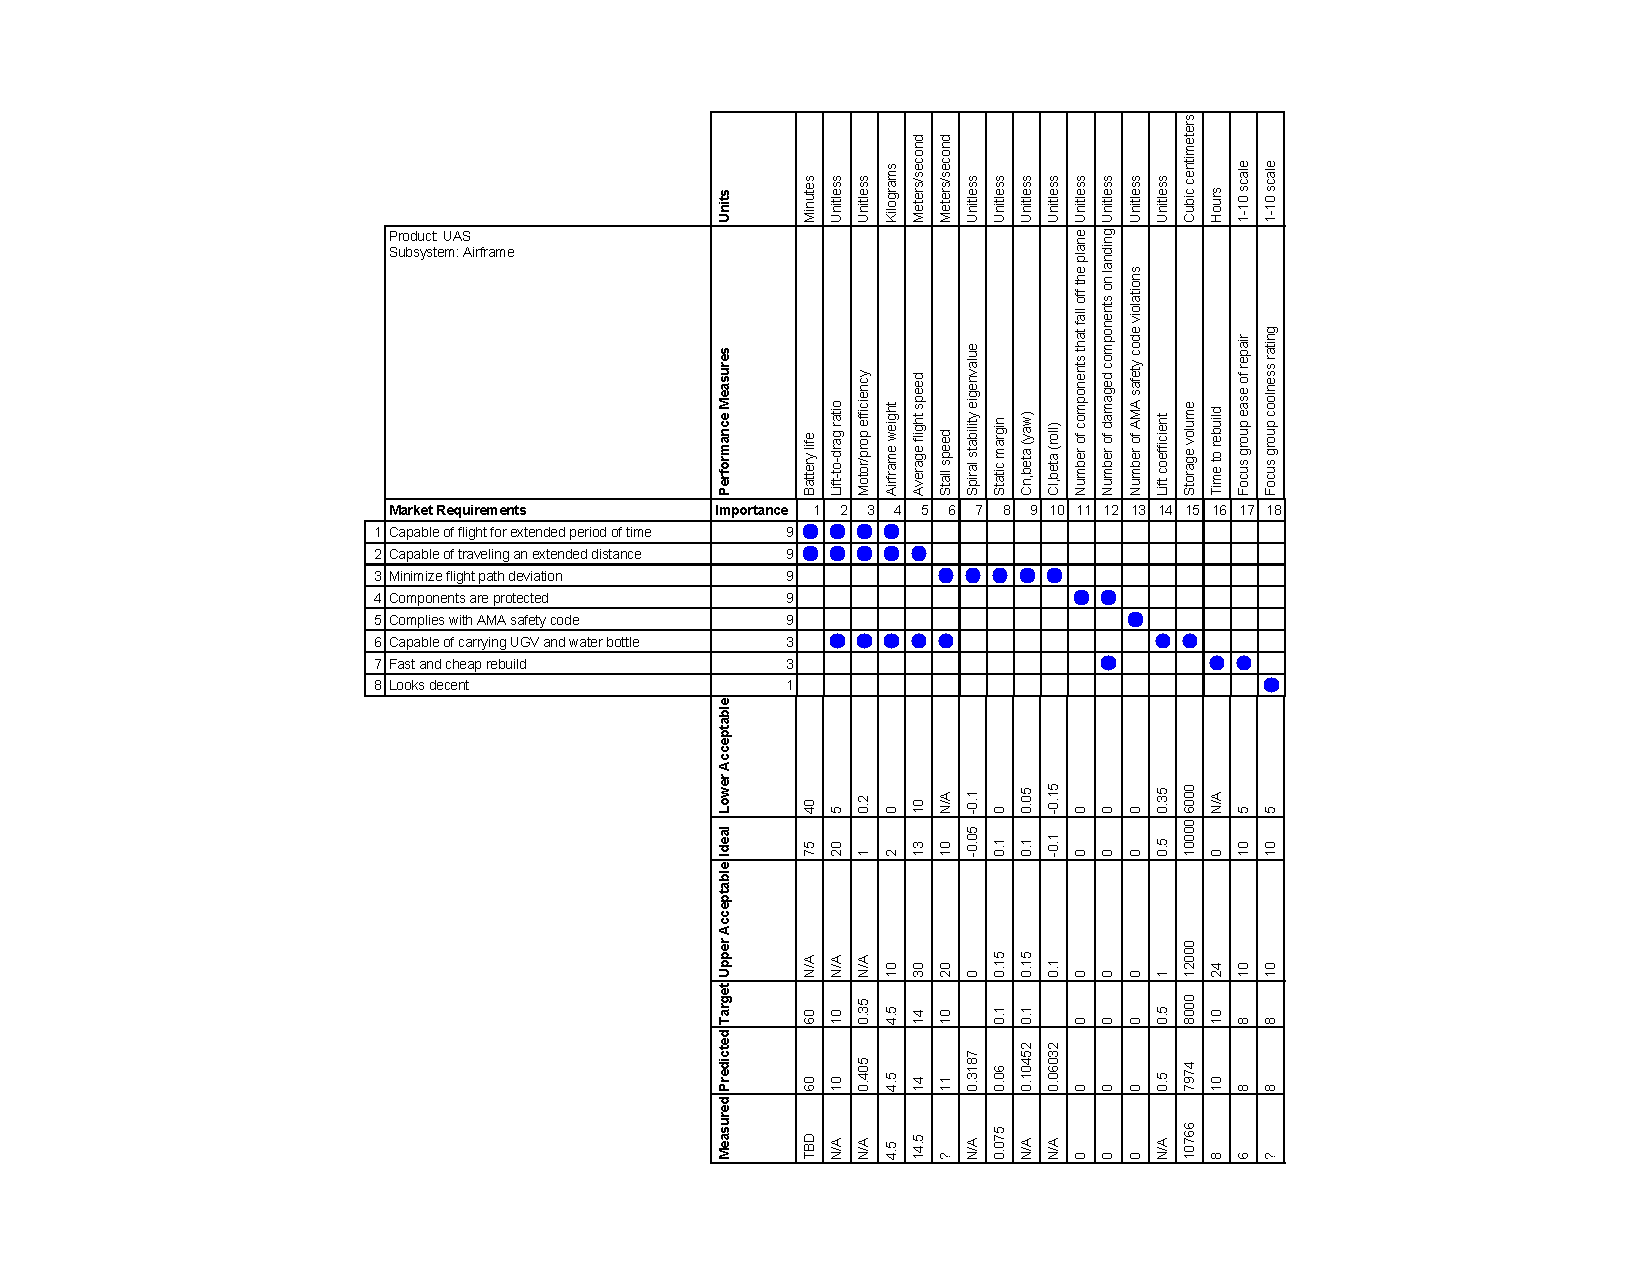
\includegraphics[width=0.8\textwidth]{reqmatrix.pdf}
	\caption{The updated requirements matrix for the airframe subsystem, with section E included (target, predicted and measured values for performance measures.)}
	\label{fig:reqmatrix}
\end{figure}


\end{document}
